\chapter{Appendix A: Formatting Examples}
%%% Ugly version requires Appendix A:, seems redundant in pretty version

%% Blow up counters for toc, lo(tfe) style examples. Probably not useful in real thesis
\setcounter{figure}{66}
\setcounter{table}{13}
\setcounter{equation}{41}
This appendix is included to show how appendices work, blowing up of numbering, and to also serve as an easy \LaTeX\ formatting template. Despite this being an appendix, it is still numbered like a chapter.

\section{Numberings in Equations}
Additionally, a reminder of Ohm's law
\begin{equation}{\label{eq:ohms law} }
V = IR
\end{equation}\eqcaption{Ohm's Law} % this function creates a new paragraph.
\noindent shows that equation numbering has blown up. This is to show spacing on the table of contents.
 
\section{Numberings in Tables}
Table~\ref{tab:exp2} is full of nonsense data and is numbered artificially large.

\begin{table}[!ht]
	\centering
	\begin{tabular}{@{} lllll @{}} 	
		\toprule % @ signs to remove extra L R space
		\footnotesize % this will affect the table font (makse it 10pt)
		One& Two  & Three  & Four  & Five  \\
		\midrule		
		2.35& 45.87  & 9.00  & 1.00  &0.33  \\
		5.88& 48.01  & 7.85  & 2.35  & 0.45 \\
		\bottomrule
	\end{tabular}
	\caption{Another Table.}
	\label{tab:exp2}
\end{table}

\section{Numberings in Figures}
Finally, Figure~\ref{fig: boxcat} shows how figure numbers look when double digit.

\begin{figure}[!ht]
	\centering
	\footnotesize
	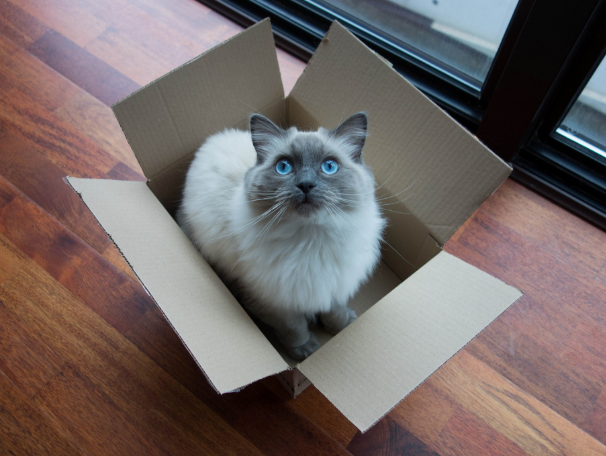
\includegraphics[height=1.5in]{boxcat}
	\caption{A boxcat in its natural environment.}
	\label{fig: boxcat}
\end{figure}\vspace{-1em} % will remove 1 white space after image - typically good

\section{Code using Minted}
Code can be added using the \verb|minted| package. The example below is for a Python example, but can be configured other ways. Note that a \verb|--shell-escape| command had to be added to the \TeX Studio build command due to peculiarities with the package. 
Additionally, the \verb|minted| \LaTeX\ package requires python to be installed with the \verb|pygments| package.
This can be done via the '\verb|py -m pip install -U pygments|' console command.

\begin{figure}[!ht]
\begin{minted}[
frame=lines,
framesep=2mm,
baselinestretch=1.2,
bgcolor=gray!13,
fontsize=\footnotesize,
linenos
]{python}
def sumPe(mirror):
    """Returns sum of all electrical power from active machines"""
    sysPe = 0.0

    # for each area
    for area in mirror.Area:
        # reset current sum
        area.cv['Pe'] = 0.0

        # sum each active machine Pe to area agent
        for mach in area.Machines:
            if mach.cv['St'] == 1:
                area.cv['Pe'] += mach.cv['Pe']

        # sum area agent totals to system
        sysPe += area.cv['Pe']

    return sysPe
\end{minted}
	\centering
	\footnotesize
	\caption{Code listing as a figure.}
	\label{fig: codeTest}
\end{figure}\vspace{-1em} % will remove 1 white space after image - typically good

Other packages exist for code insertion, but they may or may not be as pretty. Remember, as with anything, this is totally optional and voluntary...